%%%%%%%%%%%%%%%%%%%%%%%%%%%%%%%%%%%%%%%%%%%%%%%%% PREAMBLE %%%%%%%%%%%%%%%%%%%%%%%%%%%%%%%%%%%%%%%%%%%%%%%%%%

%environment setup
\documentclass[letterpaper,11pt]{article}
\usepackage[square,comma,numbers,sort&compress]{natbib}
\bibliographystyle{ieeetr}
\usepackage{amsmath}
\usepackage{graphicx}
\usepackage{url}
\usepackage{xspace}
\usepackage[left=20mm,top=20mm]{geometry}
\usepackage{hyperref}
\renewcommand{\familydefault}{\sfdefault}

%macros
\newcommand{\reffig}[1]{Figure~\ref{#1}}
\newcommand{\refsec}[1]{Section~\ref{#1}}

%%%%%%%%%%%%%%%%%%%%%%%%%%%%%%%%%%%%%%%%%%%% TITLE AND ABSTRACT %%%%%%%%%%%%%%%%%%%%%%%%%%%%%%%%%%%%%%%%%%%%%

%title
\title{Flatfielding: Spatially-Dependent Correction of Microscope High-power Field Illumination}
\author{Maggie Eminizer\\ \url{margaret.eminizer@gmail.com}\\ JHU Astropath Group}
\date{\today}
\begin{document}
\maketitle

%abstract
\abstract{This note details a method for correcting systematic variations in the illumination of multiplexed immunofluorescence microscopy images. The variations are measured using regions of image layers that are free of empty background as determined using a thresholding and masking procedure. The illumination flux observed in these regions is averaged over a large number of images, and the resulting variation pattern is smoothed to retain only the large-scale effects. The spatially-dependent corrections are defined as the ratios of these average flux patterns to their mean values in each image layer. The effect of applying these corrections is characterized using a set of 45,384 melanoma tissue images collected at the Johns Hopkins Hospital using an Akoya Biosciences Vectra 3.0 digital microscope. It is shown that the illumination of the tissue depicted in these images initially varies with an average standard deviation of 4.2\% relative flux in systematic patterns for each image layer, and that applying the corrections reduces the variation to an average standard deviation of 1.0\% relative flux in more random patterns.}

%%%%%%%%%%%%%%%%%%%%%%%%%%%%%%%%%%%%%%%%%%% INTRODUCTION SECTION %%%%%%%%%%%%%%%%%%%%%%%%%%%%%%%%%%%%%%%%%%%%
\section{Introduction}
\label{sec:introduction}

The Astropath group's work in quantifying patient outcomes from cancer immunotherapies is largely driven by analysis of multiplexed immunofluorescence microscopy images. As the group maintains focus on scaling up to curate and analyze large datasets representing multiple types of cancers contributed by a variety of primary sources or collaborators, a major push continues to be performing as much of that image analysis as possible in an automated fashion. It is therefore imperative that the image data themselves are of a very high quality, corrected for subtle effects that may adversely impact how individual images are related to one another to represent an entire microscope slide, or how the contents of those slides may be identified by automated algorithms as cells expressing certain immunofluorescence markers of interest. This note discusses a method developed to perform a low-level initial correction to the illumination of raw microscope images, and details the effect of applying this correction to an example dataset. 

%%%%%%%%%%% Flatfielding in general subsection
\subsection{Flatfielding in general}
\label{ssec:flatfielding_in_general}

The microscopes used in the Astropath group's analyses all collect light reflected off a sample illuminated by an external light source. Nonuniformities in the microscope optical path and other aspects of the methods by which slides are illuminated inherently introduce a type of systematic noise that appears as variations in the amount of illumination flux recorded at certain points in each collected image. These effects, which make some image regions brighter on average than others, tend to be especially pronounced at the edges of images, and are known interchangeably by terms including ``intensity nonuniformity,'' ``uneven shading,'' ``vignetting,'' or simply ``illumination variation'' \cite{doi:10.1111/jmi.12178}. The term ``flat field correction'' (or ``flatfielding'') refers to procedures designed to minimize these systematic illumination variations as they appear in high-power field (HPF) fluorescence microscopy images. 

Although the effects of uneven illumination may barely be noticeable within single images or during qualitative image analysis, they become much more problematic when large groups of images are analyzed, or when highly quantitative analysis depending entirely on pixel illumination flux content is performed. The Astropath group's procedure for aligning and stitching single HPF images together to represent a single high-magnification image of an entire slide is an example of such a flux-dependent quantitative analysis that would be adversely affected by certain regions of HPF images being brighter in general than others \cite{Heshy}. Other methods currently in development for automated segmentation of cells and quantitative pathology will also likewise depend on reliable measurements of illumination flux.

Methods for correction of the type of illumination variation in question have long existed, and are often built into digital microscopy image analysis platforms like CellProfiler \cite{Carpenter2006}, or even directly into automated microscope imaging procedures. These correction methods can generally be separated into the two categories of ``a-priori,'' referring to corrections derived from calibration materials imaged through the same methods as the samples of interest, and ``a-posteriori,'' referring to corrections determined only from the images of interest themselves \cite{18770694}. A-priori methods are particularly limited in effectiveness for applications in digital, high-throughput, fluorescence microscopy, because they require time and infrastructue investment in additional imaging of reference samples, the reference samples themselves can be nontrivial to prepare such that they fluoresce identically to biological samples, and because additional digital noise beyond optical effects may impact illumination variation \cite{doi:10.1111/jmi.12178}.

A-posteriori methods have therefore been developed using a variety of approaches in the 21st century, including modeling additive and multiplicative noise components and fitting the model to data by minimizing the entropy of the corrected image \cite{PMID:10692132} or filtering images for low-frequency illumination variations and correcting the pattern observed at this frequency \cite{Leong619}. Authors have also made important distinctions between illumination variation affecting slides as a whole as opposed to just the tissue or cells within an image \cite{Carpenter2006}. The method the Astropath group has developed is a-posteriori by design, and uses large samples of images of interest to measure and correct large-scale illumination variation within these images' tissue regions. The advantages of this approach are that no additional imaging of calibration samples is necessary, and that the measured corrections are unbiased to regions of images that show only background and not the tissue used for pathological analysis.

%%%%%%%%%%% Work already performed subsection
\subsection{Work already performed}
\label{ssec:work_already_performed}

The Astropath group's investigations of systematic illumination variation effects began in 2017, when substantial effects were noticed in Tissue Microarray (TMA) and deep tissue microscope images. In the first version of the work, documented in \cite{Alex_flatfielding_1}, an a-priori method was used to model the effects, wherein a slide of light diffusing material was imaged using identical methods to the slides of interest. The composite image layers, unmixed from their initial component layers, were normalized by their mean illumination flux, resulting in the pattern shown on the upper left-hand side of \reffig{fig:first_flatfielding} for the DAPI layer of the unmixed image. This pattern was fit with a two-dimensional, second degree polynomial function, shown on the upper right-hand side of \reffig{fig:first_flatfielding}. The flux at each pixel in the first layer of the full individual component IM3 image was then divided by the associated value of the function fitted to the unmixed DAPI layer, and a resulting decrease in the systematic illumination variation was observed, as shown in the lower plot in \reffig{fig:first_flatfielding}. Similar methods using a third-degree polynomial fit were applied to the other layers of the unmixed images, as well as the individual component IM3 layers, with varying results. It was concluded that a polynomial fit was likely insufficient to describe the illumination variations in all image layers.

\begin{figure}[!ht]
\centering
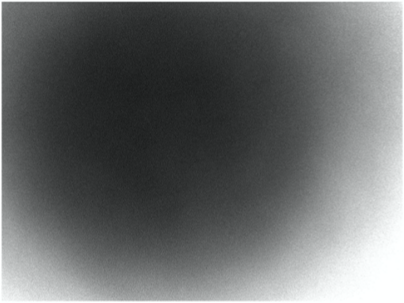
\includegraphics[width=0.45\textwidth]{images/first_unmixed_DAPI_meanimage}
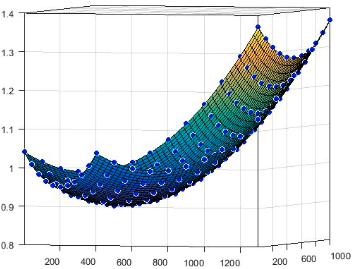
\includegraphics[width=0.45\textwidth]{images/first_DAPI_meanimage_polynomial_fit}
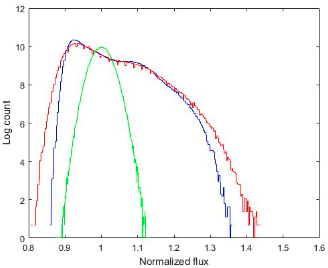
\includegraphics[width=0.45\textwidth]{images/first_DAPI_meanimage_corrected_flux}
\caption{\footnotesize Upper left: Illumination flux pattern observed in the unmixed DAPI layer of an imaged light diffuser. Upper right: Two-dimensional, second-degree polynomial fitted to the mean-normalized flux pattern pictured in the upper left figure. Lower: Histogram of log pixel counts vs. mean-normalized flux for the light diffuser image's unmixed DAPI layer (in red), first component IM3 layer (in blue), and first component IM3 layer after pixelwise division by the polynomial shown in the upper right plot (in green); the applied correction has reduced the systematic illumination variation to more Gaussian noise. Figures from \cite{Alex_flatfielding_1}.}
\label{fig:first_flatfielding}
\end{figure}

After these initial investigations, the decision was made to correct illumination variations in images in the raw IM3 component layers rather than in the unmixed composite image layers, and a new a-posteriori method was devloped to model the effects, as documented in \cite{Alex_flatfielding_2}. In this method, the flatfielding corrections were determined by making a single, multi-layer, average raw image from a set of 7,358 HPFs, smoothing the layers of the mean image with a Gaussian filter of standard deviation $\sigma=100$ pixels to retain only the large-scale pattern, and dividing this smoothed mean image by the mean average flux value layer-by-layer so that the corrections did not change the overall illumination of each image layer. It was found that this method resulted in consistent illumination variation patterns, shown in \reffig{fig:second_flatfielding}, correlated within layers contributing to the same broadband filter region (raw layers 1-9, 10-18, 19-25, 26-32, and 33-35 for the DAPI, FITC, Cy3, Texas Red, and Cy5 unmixed spectral components, respectively).

\begin{figure}[!ht]
\centering
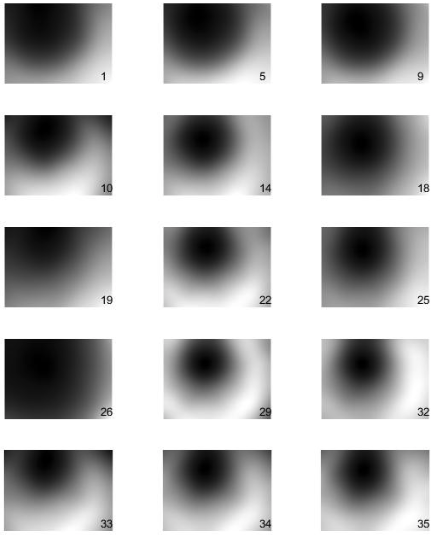
\includegraphics[width=0.8\textwidth]{images/second_flatfield_image_layers}
\caption{\footnotesize Selected layers of the flatfield image from \cite{Alex_flatfielding_2}, stretched from minimum to maximum mean-normalized flux, in the first, middle, and last layer of each broadband filter region as labeled. The patterns are fairly consistent between each broadband filter break. Layer 26, the first layer in the Texas Red region, was not brightly illuminated for the melanoma tissue samples used, and represents an outlier in this and other investigations.}
\label{fig:second_flatfielding}
\end{figure}

After using this new model for some time to correct HPF illumination, it was discovered \cite{Ben_flatfielding_1} that the algorithm implemented in the inForm software package \cite{Kramer2018} used to phenotype cells for pathology was over-identifying cells of a certain type in some more recently-collected samples, in a pattern similar to that of the original flatfield correction images. Updated flatfield correction models were developed using the same averaging, smoothing, and normalizing method as in \cite{Alex_flatfielding_2} for different subsets of the data separated by time of collection (or ``Batch''), and it was discovered that changing the lightbulb in the microscope between batches had a significant effect on the pattern of illumination variation, as shown in \reffig{fig:third_flatfielding}. 

\begin{figure}[!ht]
\centering
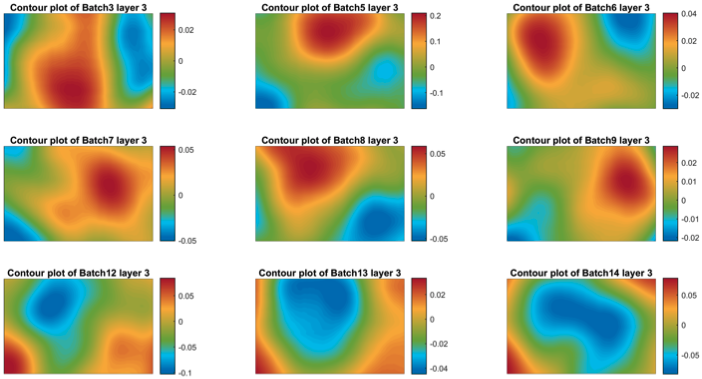
\includegraphics[width=0.9\textwidth]{images/third_flatfield_differences}
\caption{\footnotesize Differences in the third unmixed image layer between the normalized mean images computed independently for each batch and the original flatfield correction image measured in \cite{Alex_flatfielding_2} using a subset of the Batch3 data. These images showed that the illumination variations changed between batches, and especially for batches 12 and 13-14, before the collection of which the lightbulb in the microscope was replaced. Figures from \cite{Ben_flatfielding_1}.}
\label{fig:third_flatfielding}
\end{figure}

At this point the decision was made to measure and correct for the illumination variations independently for each batch of images collected. The work documented in \cite{Ben_flatfielding_1} also gave the first look at the illumination variations in samples collected with the Vectra Polaris imaging system as opposed to the Vectra 3.0 digital microscope, showing that the overall amount of variation was less for the Vectra Polaris, and the patterns were different in shape, likely due to the Vectra Polaris using an LED array rather than a lightbulb for slide illumination. This comparison was made in greater detail in \cite{Ben_flatfielding_2} where two component-layer mean image models were computed from sets of 10,000 HPFs collected with the Vectra 3.0 and Vectra Polaris microscopes. The corrections were applied to sets of 10,000 independent HPF datasets from each microscope, and the uncorrected and corrected images were unmixed using inForm and their own average images were compared. It was discovered that applying the flatfield corrections greatly reduced the overall illumination variation in the average unmixed images for both the Vectra 3.0 and Vectra Polaris microscopes, as shown in \reffig{fig:fourth_flatfielding}. To date this type of model of the average of large sets of images is used for correcting illumination variation before unmixing.

\begin{figure}[!ht]
\centering
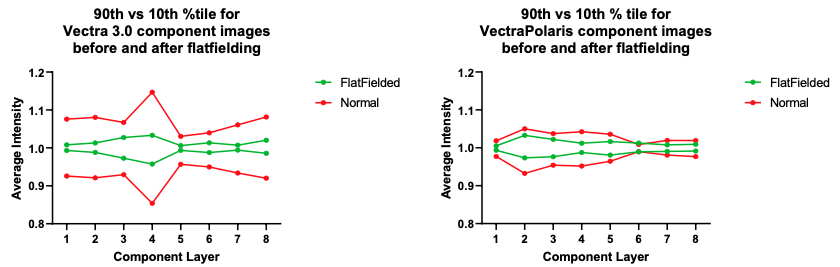
\includegraphics[width=0.9\textwidth]{images/fourth_flatfield_impact}
\caption{\footnotesize 10th and 90th percentile illumination flux relative to the layer mean in smoothed, unmixed average images before and after application of flatfielding corrections for data collected with the Vectra 3.0 and Vectra Polaris microscopes. The flatfielding corrections and the averages of the images to which they were applied were determined using independent sets of 10,000 HPFs each. Applying flatfield corrections of this type of smoothed, normalized, mean image layers reduced the overall illumination variation observed for images from both microscopes. Figures from \cite{Ben_flatfielding_1}.}
\label{fig:fourth_flatfielding}
\end{figure}

%%%%%%%%%%% This work subsection
\subsection{This work}
\label{ssec:this_work}

It is the goal of the work documented in this note to provide the most detailed and highest quality measurements of the illumination variation and associated flatfield corrections yet made by the Astropath group. To this end, an additional step has been implemented in the flatfielding procedure to only average over regions of images that are determined to show tissue, since the inclusion of empty background regions in many of the images over which the average is taken may bias measurements away from noise specifically affecting the tissue used for quantitative clinical pathology further down the line. A secondary goal of this work is to re-implement the analysis pipeline in python, an open-source programming language, and to develop a single software package that is not only easy to use but also able to scale up to even higher throughput without complicating analysis or prohibitively increasing runtime.

Here are the details on the datasets I used to make these measurements.

Here is an overview of the rest of the note.

%%%%%%%%%%%%%%%%%%%%%%%%%%%%%%%%%%%%%%%%%%% IMAGE MASKING SECTION %%%%%%%%%%%%%%%%%%%%%%%%%%%%%%%%%%%%%%%%%%%
\section{Image Masking}
\label{sec:image_masking}

%%%%%%%%%%% Determining background flux thresholds subsection
\subsection{Determining background flux thresholds}
\label{ssec:determining_background_flux_thresholds}

%%%%%%%%%%% Producing image masks subsection
\subsection{Producing image masks}
\label{ssec:producing_image_masks}

%%%%%%%%%%%%%%%%%%%%%%%%%%%%%%%%%% MEASURING FLATFIELD CORRECTIONS SECTION %%%%%%%%%%%%%%%%%%%%%%%%%%%%%%%%%%
\section{Measuring Flatfield Corrections}
\label{sec:measuring_flatfield_corrections}

%%%%%%%%%%% Stacking masked images subsection
\subsection{Stacking masked images}
\label{ssec:stacking_masked_images}

%%%%%%%%%%% Averaging and smoothing subsection
\subsection{Averaging and smoothing}
\label{ssec:averaging_and_smoothing}

%%%%%%%%%%%%%%%%%%%%%%%%%%%%%%%%%%%%%%%%%%%%%% RESULTS SECTION %%%%%%%%%%%%%%%%%%%%%%%%%%%%%%%%%%%%%%%%%%%%%%
\section{Results}
\label{sec:results}

%%%%%%%%%%% Flatfield images subsection
\subsection{Flatfield images}
\label{ssec:flatfield_images}

%%%%%%%%%%% Reduction in illumination variation subsection
\subsection{Reduction in illumination variation}
\label{ssec:reduction_in_illumination_variation}

%%%%%%%%%%%%%%%%%%%%%%%%%%%%%%%%%%%%%%%%%%%%%% SUMMARY SECTION %%%%%%%%%%%%%%%%%%%%%%%%%%%%%%%%%%%%%%%%%%%%%%
\section{Summary}
\label{sec:summary}

%%%%%%%%%%%%%%%%%%%%%%%%%%%%%%%%%%%%%%%%%%%%%%% BIBLIOGRAPHY %%%%%%%%%%%%%%%%%%%%%%%%%%%%%%%%%%%%%%%%%%%%%%%%
\bibliography{references}

\end{document}